%%%%%%%%%%%%%%%%%%%%%%%%%%%%%%%%%%%%%%%%%
% Beamer Presentation
% LaTeX Template
% Version 1.0 (10/11/12)
%
% This template has been downloaded from:
% http://www.LaTeXTemplates.com
%
% License:
% CC BY-NC-SA 3.0 (http://creativecommons.org/licenses/by-nc-sa/3.0/)
%
%%%%%%%%%%%%%%%%%%%%%%%%%%%%%%%%%%%%%%%%%

%----------------------------------------------------------------------------------------
%	PACKAGES AND THEMES
%----------------------------------------------------------------------------------------

\documentclass{beamer}

\mode<presentation> {
\usetheme{Madrid}
\usecolortheme{orchid}
}

\usepackage{graphicx} % Allows including images
\usepackage{booktabs} % Allows the use of \toprule, \midrule and \bottomrule in tables

\setbeamertemplate{footline}
{
  \leavevmode%
  \hbox{%
  \begin{beamercolorbox}[wd=.333333\paperwidth,ht=2.25ex,dp=1ex,center]{author in head/foot}%
    \usebeamerfont{author in head/foot}\insertshorttitle
  \end{beamercolorbox}%
  \begin{beamercolorbox}[wd=.333333\paperwidth,ht=2.25ex,dp=1ex,center]{title in head/foot}%
    \usebeamerfont{title in head/foot}\insertsection
  \end{beamercolorbox}%
  \begin{beamercolorbox}[wd=.333333\paperwidth,ht=2.25ex,dp=1ex,right]{date in head/foot}%
    \usebeamerfont{date in head/foot}\insertshortdate{}\hspace*{2em}
    \insertframenumber{} / \inserttotalframenumber\hspace*{2ex}
  \end{beamercolorbox}}%
  \vskip0pt%
}
%\definecolor{Pearl}{rgb}{0.94,0.92,0.84}


\definecolor{Pearl}{rgb}{0.95,0.93,0.87}

%----------------------------------------------------------------------------------------
%	TITLE PAGE
%----------------------------------------------------------------------------------------

\title[Statistical Learning with Visualization]{Introduction to Statistical Learning with Visualization} % The short title appears at the bottom of every slide, the full title is only on the title page
\vspace{2cm}
\author{Dr YINGHUI WEI} % Your name
\institute[UoP] % Your institution as it will appear on the bottom of every slide, may be shorthand to save space
{
\medskip
Email: yinghui.wei@plymouth.ac.uk % Your email address
}
\date{\empty} % Date, can be changed to a custom date

\begin{document}
\begingroup
\setbeamercolor{background canvas}{bg=Pearl}
\begin{frame}
\titlepage % Print the title page as the first slide
\end{frame}

\begin{frame}
\frametitle{Overview} % Table of contents slide, comment this block out to remove it
\tableofcontents % Throughout your presentation, if you choose to use \section{} and \subsection{} commands, these will automatically be printed on this slide as an overview of your presentation
\end{frame}

%----------------------------------------------------------------------------------------
%	PRESENTATION SLIDES
%----------------------------------------------------------------------------------------





\frame{
\frametitle{Real-life data visualization}

Click on each item below:
\begin{itemize}
  \item \href{http://www.ons.gov.uk/ons/rel/tourism/tourism-satellite-account/the-economic-importance-of-tourism--uk-tourism-satellite-account-2012/sto-infographic.html}{ONS: infographic for TSA}
  \item \href{http://www.ons.gov.uk/ons/rel/lifetables/historic-and-projected-data-from-the-period-and-cohort-life-tables/2012-based/info-surviving-to-age-100.html}{ONS: Survival to age 100}
  \item \href{https://www.theguardian.com/membership/2014/sep/10/best-infographic-graphic-design}{Guardian website: The best of infographics}
  \item  \href{http://news.nationalgeographic.com/2015/09/150922-data-points-visualization-eye-candy-efficiency/}{BBC website: taking data visualization eye candy to efficiency}

  \item \href{http://www.bankofengland.co.uk/research/Pages/onebank/dataviscomp.aspx}{Bank of England: data visualization competition}
  \item  \href{http://climate.nasa.gov/evidence/}{NASA: Global Climate Change}
\end{itemize}
}

\section{Visualization}
\frame{
\frametitle{Introduction to Visualization}

\begin{itemize}
  \item Visualizations help people see things that were not obvious to them by looking at the raw data.

  \item Even when data volumes are very large, patterns can be spotted quickly and easily.

  \item Visualizations convey information in a universal manner and make it simple to share ideas with others.
\end{itemize}
}



\frame{
\frametitle{Graphs}
Some widely used graphs:
\begin{itemize}
  \item Bar
  \item Boxplot
  \item Histogram
  \item Pie
  \item Scatter plot
  \item Contour plot
  \item Line graphs
  \item Heat map
\end{itemize}
}

\frame{
\frametitle{Recommended Text for Visualization}

\centering
\includegraphics[scale=0.7]{figures/graphics}

\vspace{0.2cm}

\url{http://www.cookbook-r.com/}

%More resources on visualization:
%
%\begin{itemize}
%  \item \url{http://rgraphgallery.blogspot.co.uk/}
%  \item \url{http://www.ling.upenn.edu/~joseff/rstudy/summer2010_ggplot2_intro.html}
%  \item \url{http://docs.ggplot2.org/current/}
%\end{itemize}


}
\section{Examples for Visualization}


\frame{

\frametitle{Visualization Example - Birth Weight}

In this application, we investigate risk factors associated with low birth weight.

\begin{center}
\pause 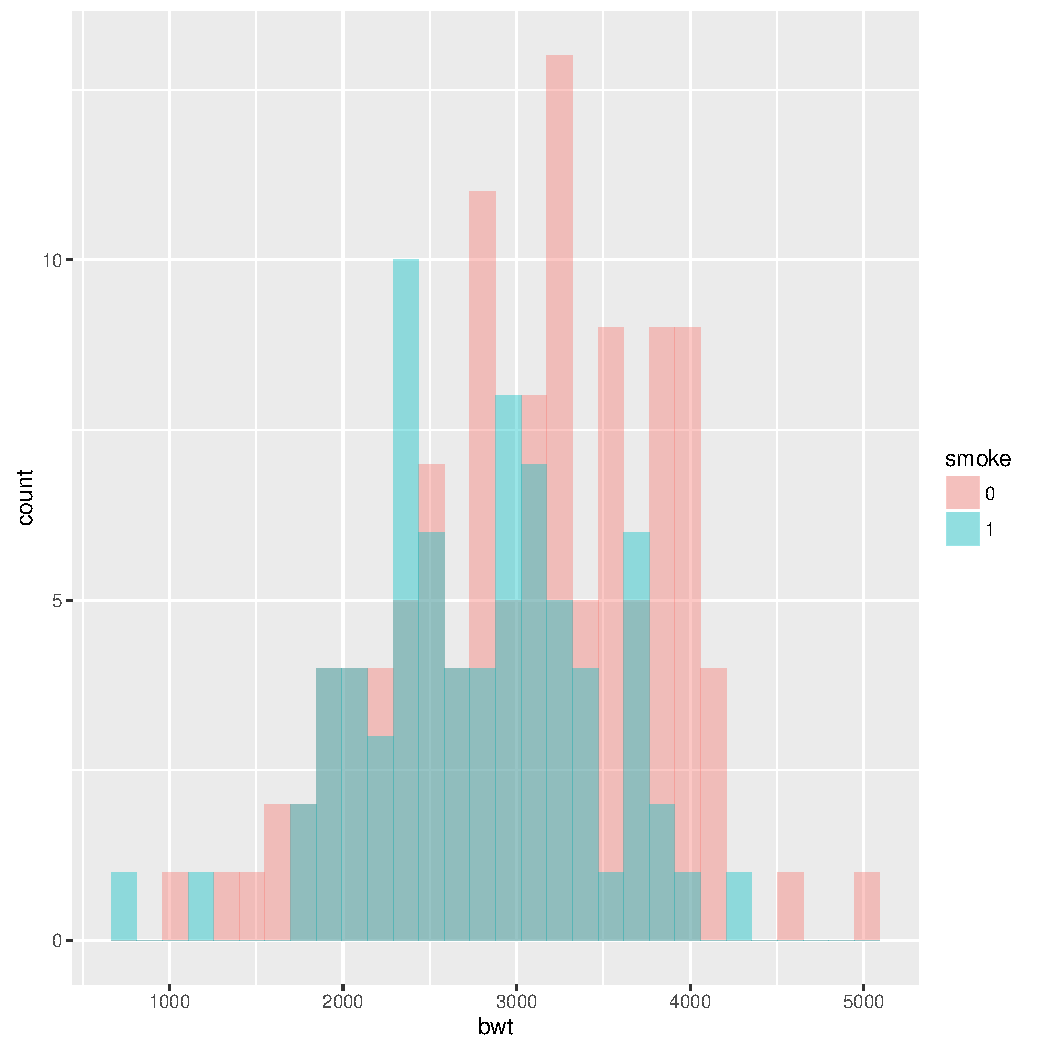
\includegraphics[scale=0.3]{figures/histogram}
\end{center}
}


\frame{

\frametitle{Visualization Example - Birth Weight}

Box plot

\begin{center}
\pause 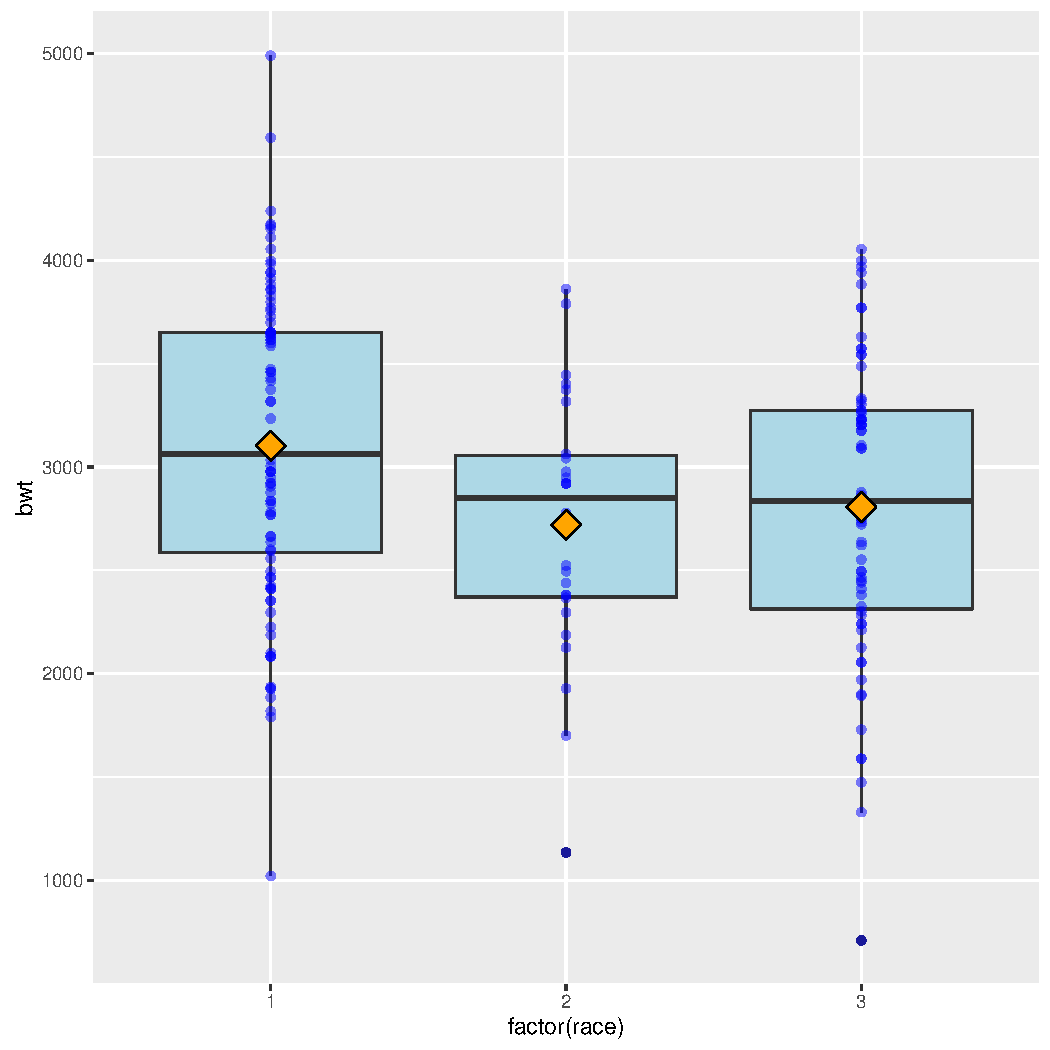
\includegraphics[scale=0.3]{figures/boxplot}
\end{center}
}


\frame{
\frametitle{Visualization Example - Birth Weight}

Scatter plot

\begin{center}
\pause 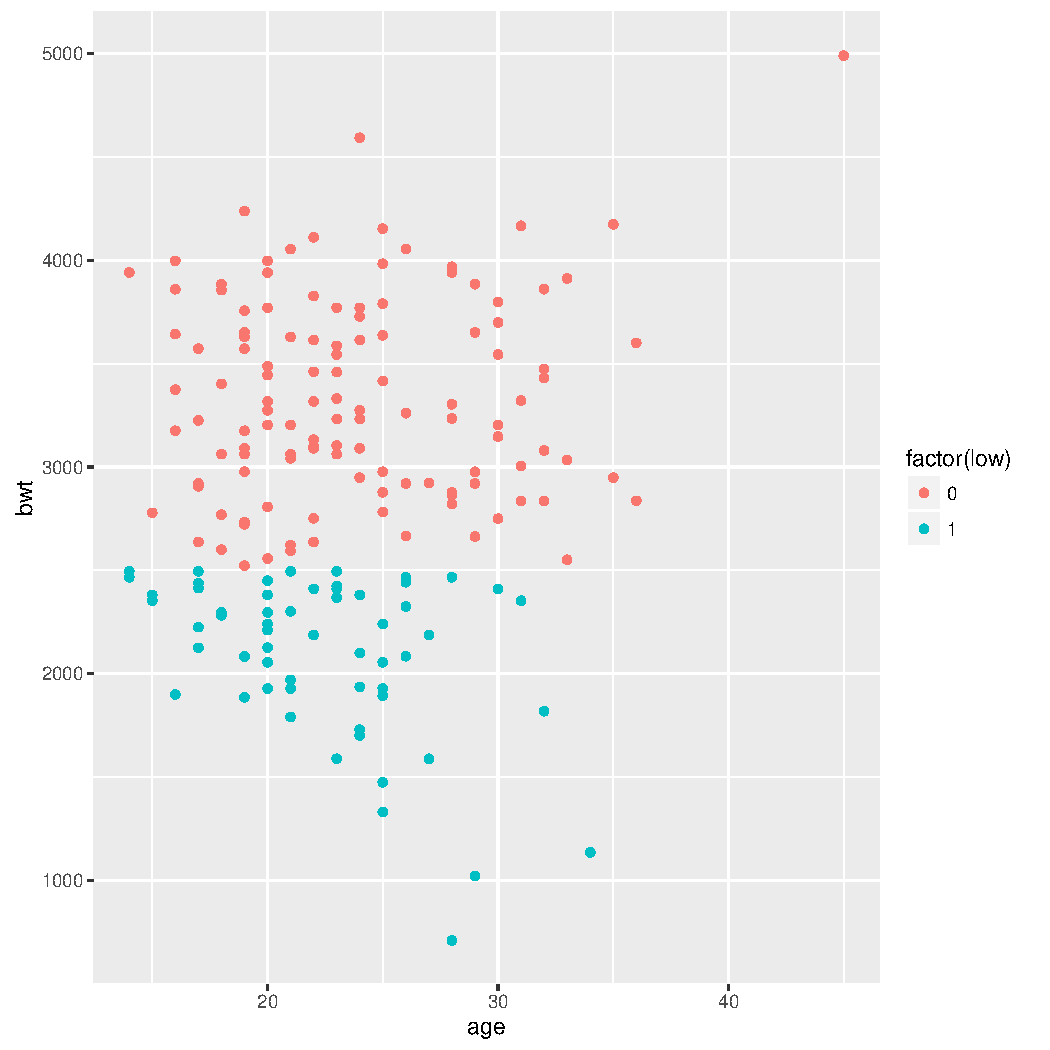
\includegraphics[scale=0.3]{figures/scatter}
\end{center}
}



\frame{
\frametitle{Visualization Example  - Wage}
In this application, we examine a number of factors that relate to wages for a group of
males from the Atlantic region of the United States. In particular, we wish
to understand the association between an employee's age and education, as
well as the calendar year, on his wage.

\begin{center}
\pause 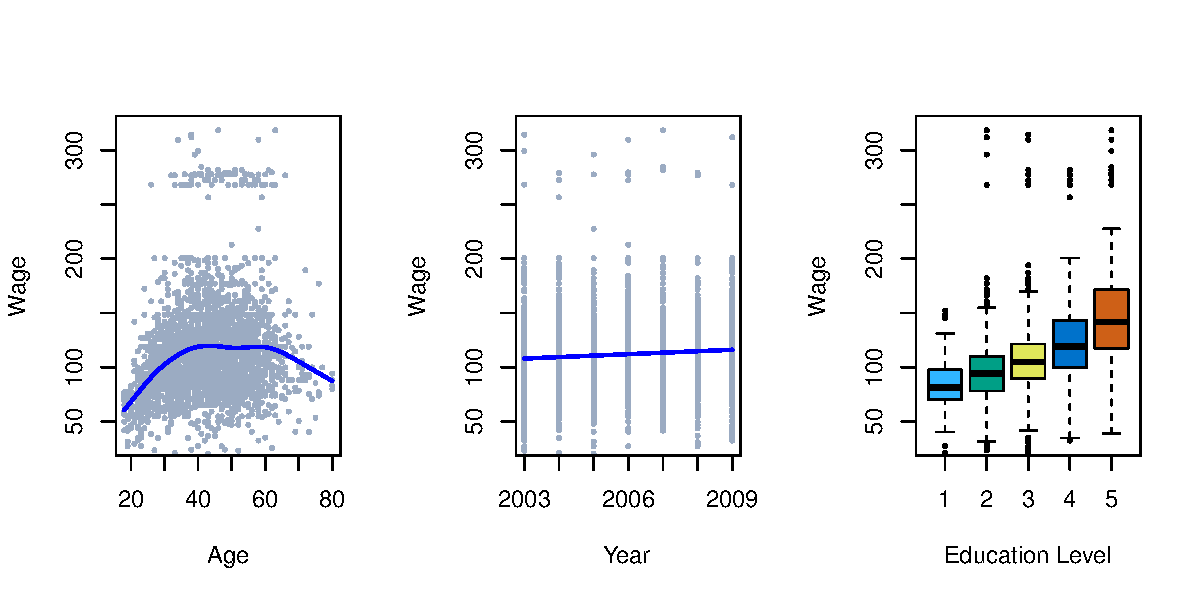
\includegraphics[scale=0.55]{figures/wage}
\end{center}

}

\frame{
\frametitle{Visualization Example - Gene Expression Data}
In this application, we consider the a data set consisting of 6,830 gene expression measurements
for each of 64 cancer cell lines. Instead of predicting a particular output
variable,  we are interested in determining whether there are groups,  or
clusters, among the cell lines based on their gene expression measurements.

}


\frame{

\frametitle{Visualization Example - Gene Expression Data}

\begin{center}
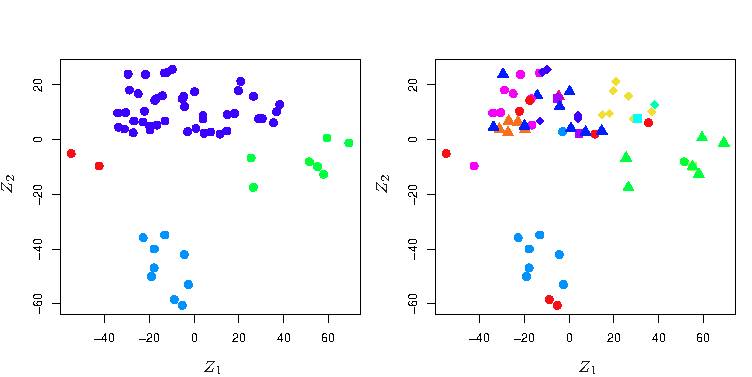
\includegraphics[scale=0.6]{figures/gene}
\end{center}
Left: Representation of the NCI60 gene expression data set in
a two-dimensional  space, $Z_1$ and $Z_2$ . Each point corresponds to one of the 64
cell lines. There appears to be four groups of cell lines, which we have represented
using different colors. Right: Same as left panel except that we have represented
each of the 14 different types of cancer using a different colored symbol. Cell lines
corresponding to the same cancer type tend to be nearby in the two-dimensional
space.

}




\section{Statistical Learning}
\frame{
\frametitle{Introduction to Statistical Learning}
\begin{itemize}
  \item Statistical learning refers to a set of tools for modelling and understanding complex data sets.
  \item The field encompasses many methods such as \alert{regression models}, \alert{classification}, \alert{regression trees}, \alert{bagging}, \alert{random forest} and \alert{boosting methods}.
  \item With the explosion of “Big Data” problems, statistical learning has become a very hot field in medicine, engineering as well as marketing, finance, and other business disciplines.
\end{itemize}

}



\frame{
\frametitle{Recommended Text for Statistical Learning}

\noindent

\begin{minipage}{.5\textwidth}
\centering
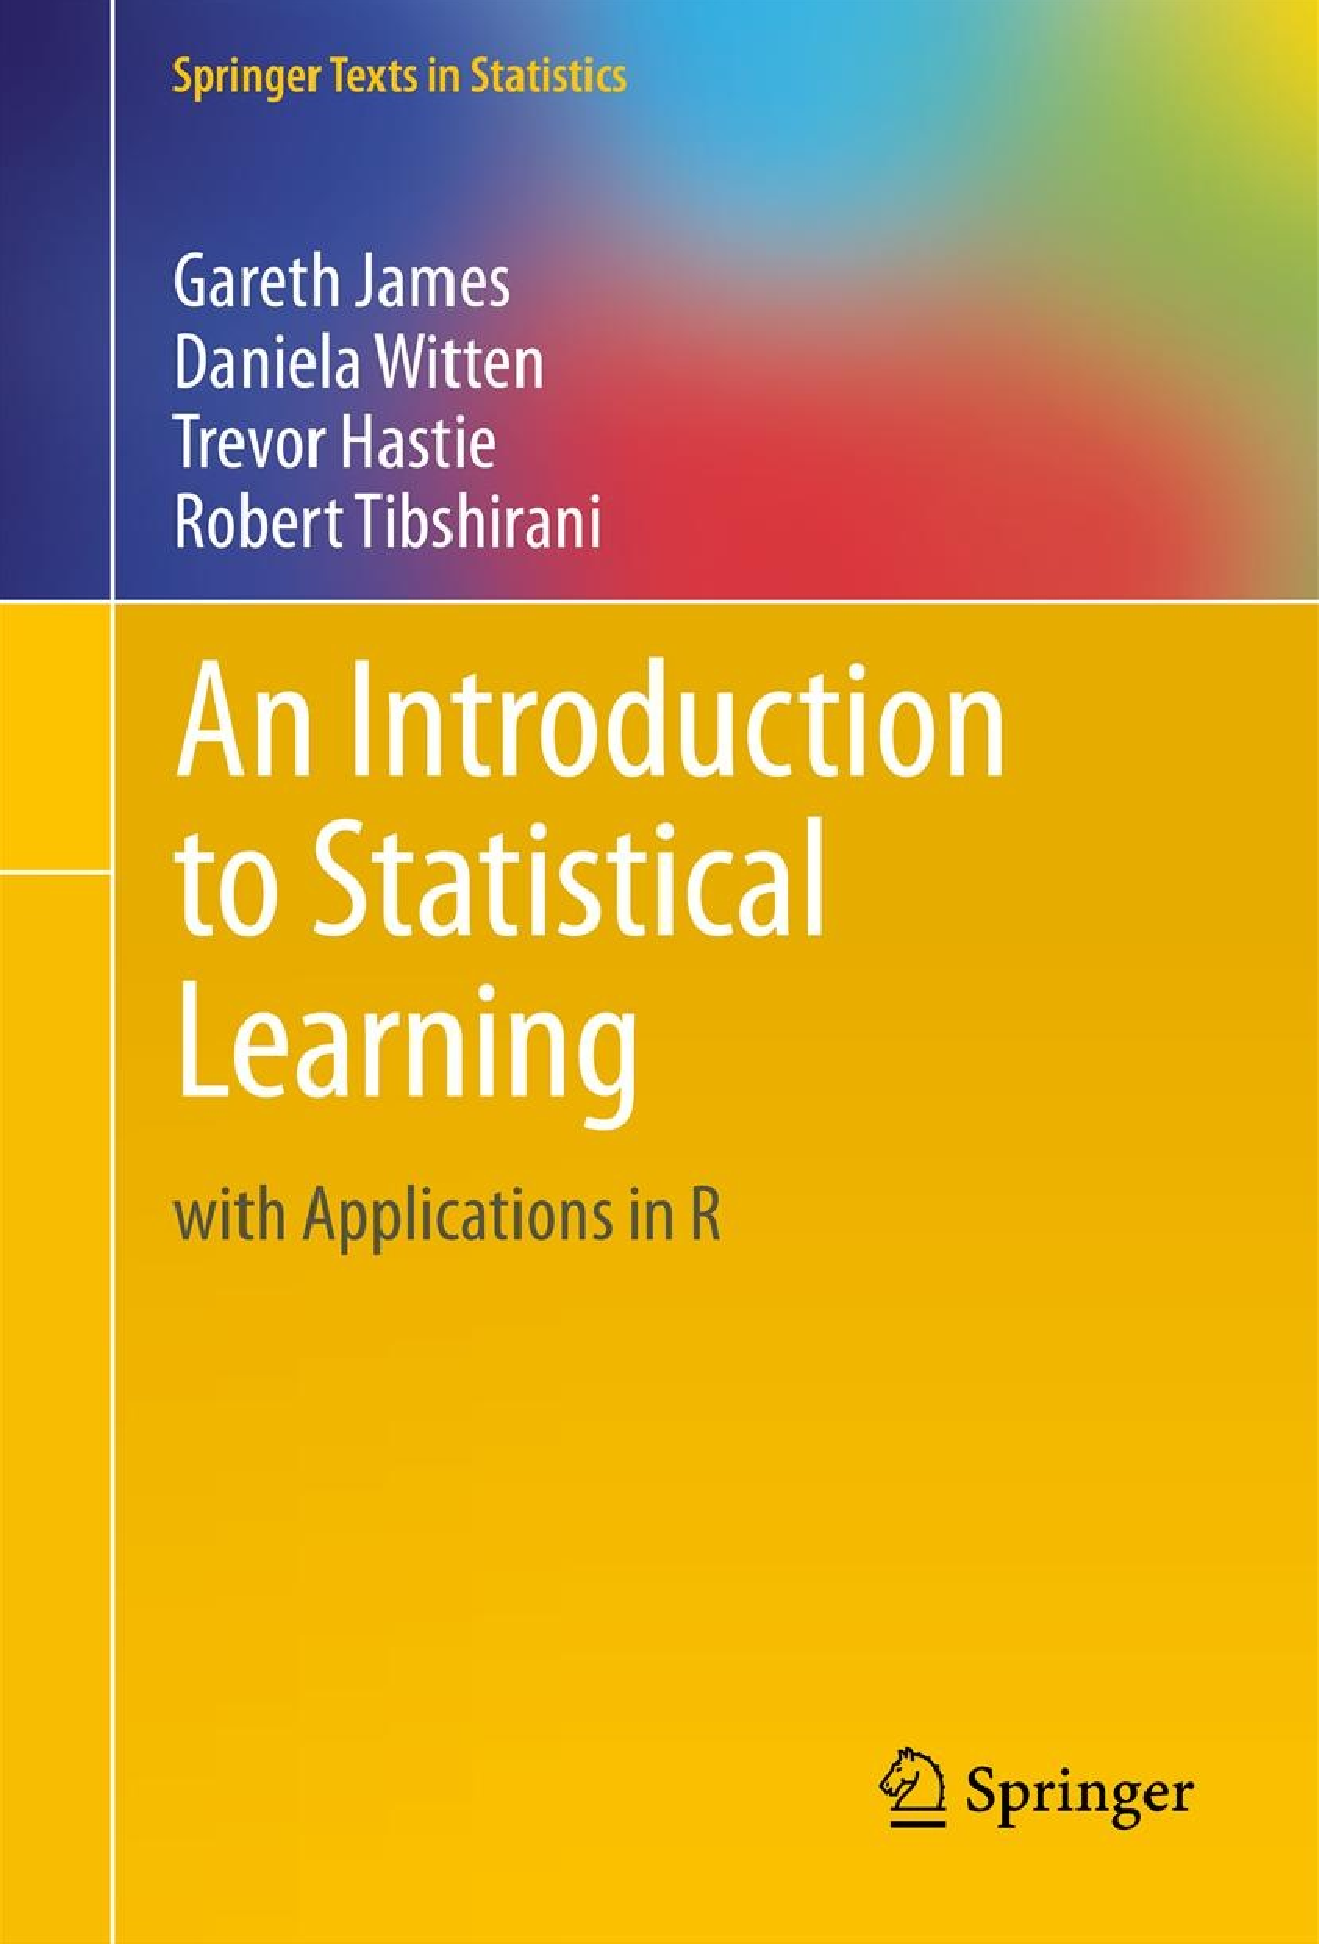
\includegraphics[scale=0.15]{figures/book}
\end{minipage}%
\begin{minipage}{0.5\textwidth}
Ch 1. Introduction\\
Ch 2. Statistical Learning\\
Ch 3. Linear Regression\\
Ch 4. Classification\\
Ch 5. Resampling Methods\\
Ch 6. Linear Model Selection and Regularization\\
Ch 7. Moving Beyond Linearity\\
Ch 8. Tree-Based Methods\\
Ch 9. Support Vectors Machines\\
Ch 10. Unsupervised Learning
\end{minipage}

\vspace{1cm}
\centering
\url{http://www-bcf.usc.edu/~gareth/ISL/index.html}
}

\frame
{\frametitle{Variables Type}

\textcolor{red}{Quantitative variables} take on numerical  values:

\begin{itemize}
  \item  Examples include a person's age, height, or income, the value of a house,
 categorical and the price of a stock.
\end{itemize}

 \vspace{0.5cm}
\textcolor{red}{Qualitative variables} take on values in one of $K$ different classes,  or categories:

\begin{itemize}
  \item  Examples include a person's gender (male or female), the brand of product purchased (brand A,  B, or C), whether a person defaults on a debt (yes or no), or a cancer diagnosis (Acute Myelogenous Leukemia, Acute Lymphoblastic Leukemia, or No Leukemia).
\end{itemize}

}


\frame
{\frametitle{Classification Questions}
\begin{itemize}
\item  A person arrives at the emergency room with a set of  symptoms
that could possibly be attributed to one of three medical conditions.
Which of the three conditions does the individual have?
\item  An online banking service must be able to determine whether or not a transaction being performed on the site is fraudulent, on the basis of the user IP address, past transaction history, and so forth.
\end{itemize}
}

\frame
{\frametitle{Classification Techniques}

There are many possible classification techniques, or classifiers, that one might use to predict a qualitative response.  Three most widely-used classifiers:

\begin{itemize}
  \item Logistic Regression
  \item Linear Discriminant Analysis
  \item K-Nearest Neighbours
\end{itemize}
}


\section{A Case Study for Statistical Learning}


\frame
{\frametitle{{\it Default} Data}

We are interested in \textcolor{red}{predicting} whether an individual will default on his or her credit card payment, on the basis of annual \textcolor{blue}{income} and monthly credit card \textcolor{blue}{balance}.

\begin{center}
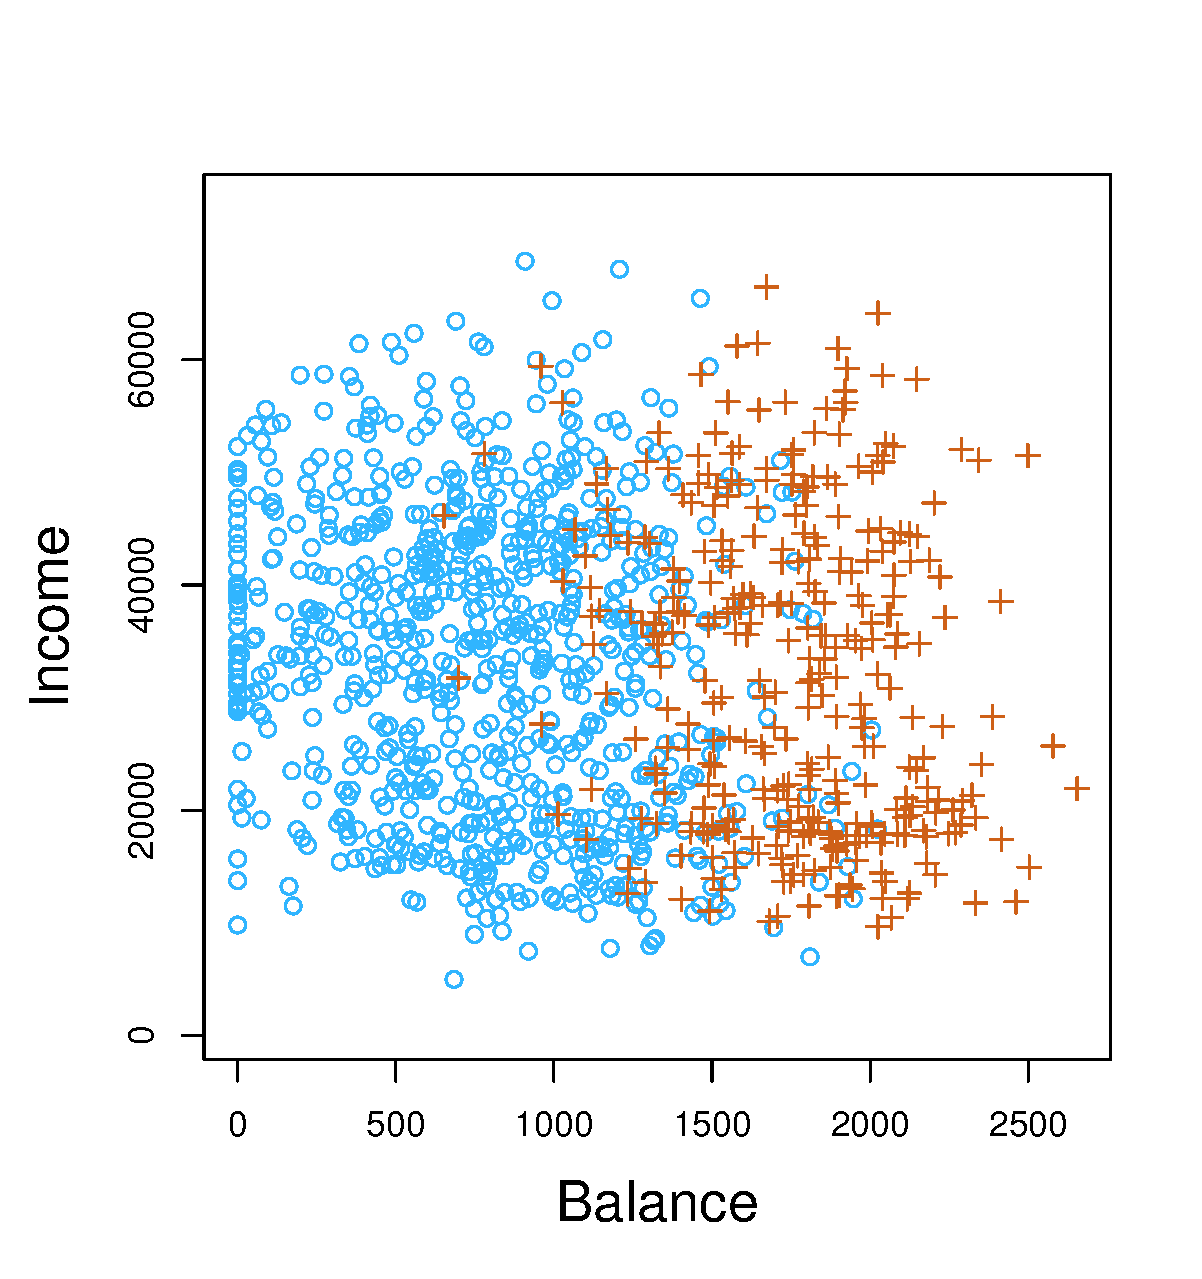
\includegraphics[scale=0.25]{figures/default}
\end{center}
\pause Which variable would you choose as a predictor of \textit{default} (orange).

}
\frame
{\frametitle{{\it Default} Data}


\begin{center}
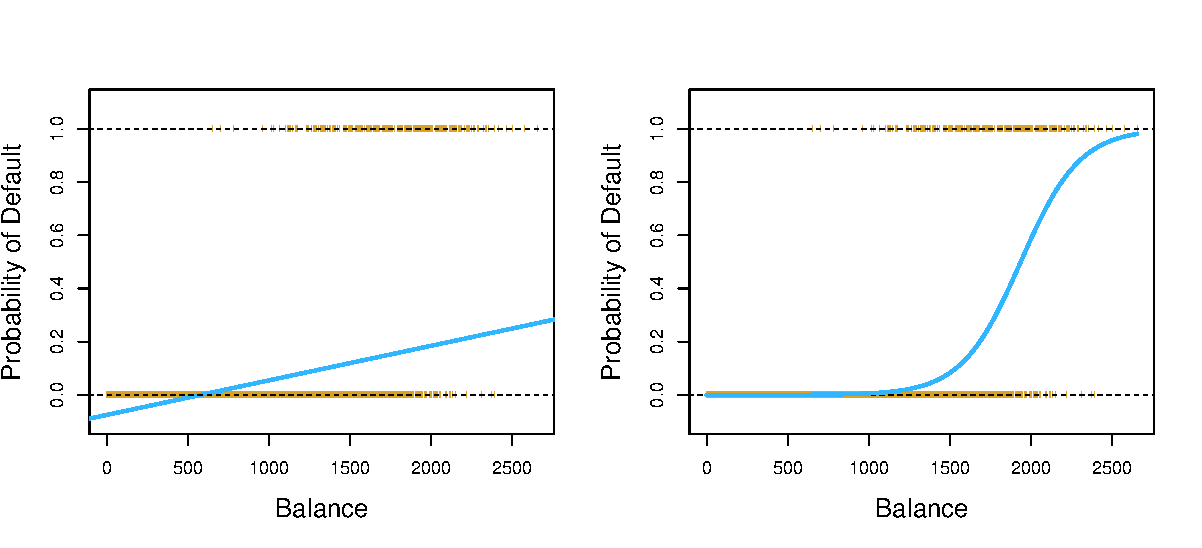
\includegraphics[scale=0.50]{figures/logistic}
\end{center}

}


\frame
{\frametitle{Model}
\begin{block}{Logistic Model}

\begin{eqnarray*}
\textrm{logit}\left(p(X)\right) &=& \beta_0 + \beta_1 X \\
\log \left(\frac{p(X)}{1-p(X)}\right) &=& \beta_0 + \beta_1 X
\end{eqnarray*}
\end{block}

\vspace{0.5cm}
\pause \begin{itemize}
\item $p(X)$ represents the \textcolor{red}{probability of success}, $p(Y=1|X)$.
\item The fraction $\displaystyle\frac{p(Y=1|X)}{1-p(Y=1|X)}$ represents the \textcolor{red}{odds} of the event.
\item Values of the odds close to 0 and $+\infty$ indicate very low and very high probabilities of default, respectively.

\end{itemize}
}

\frame
{\frametitle{Maximum Likelihood}
We use maximum likelihood to estimate the model parameters. The likelihood function is:

\[\mathcal{L}(\beta_0, \beta_1) = \prod_{i:y_i=1} p(x_i) \prod_{i:y_i=0} \left(1-p(x_i)\right).  \]

\vspace{0.5cm}
We find the estimated values of $\beta_0$ and $\beta_1$ which maximise this likelihood. The estimates can be obtained by using standard packages in R.

}

\frame{

\frametitle{Results}
For the Default data, estimated coefficients of the logistic regression model that predicts the probability of default using balance are given in the following table:



\begin{table}[h]
\begin{tabular}{l|rrrr}
\hline
 & Coefficient & Std. Error & Z-statistic & P-value \\
\hline
\alert{Intercept} & -10.6513 & 0.3612 & -29.5 & $<0.0001$ \\
\alert{Balance} & 0.0055 & 0.0002 & 24.9 & $<0.0001$ \\
\hline
\end{tabular}
\caption{Estimated coefficients in univariate logistic model  for the Default data}
\end{table}

}

\frame
{\frametitle{Making Predictions}
Once the coefficients have been estimated, it is a simple matter to compute the probability of default for any given credit card balance. For example, using the coefficient estimates given in Table 1, we predict that the default probability for an individual with a balance of \$ 1, 000 is

{\large
\begin{eqnarray*}
\hat{p}(X) &=& \frac{e^{\hat{\beta}_0+\hat{\beta}_1X}}{1 + e^{\hat{\beta}_0+\hat{\beta}_1X}}
= \frac{e^{-10.6513+0.0055 \times 1000}}{1 + e^{-10.6513+0.0055 \times 1000}}
=0.00576
\end{eqnarray*}
}
}


\frame
{
\frametitle{Multiple Logistic Regression}

We now consider the problem of predicting a binary response using multiple predictors. The multivariable logistic model is:

\[\log \left(\frac{p(X)}{1-p(X)}\right) = \beta_0 + \beta_1 X_1 + \beta_2 X_2 + \ldots + \beta_p X_p, \]

and so

\[p(X)= \frac{exp^{\beta_0 + \beta_1 X_1 + \beta_2 X_2 + \ldots + \beta_p X_p}}{1+exp^{\beta_0 + \beta_1 X_1 + \beta_2 X_2 + \ldots + \beta_p X_p}} \]
Parameters will be estimated using maximum likelihood.
}




\frame
{\frametitle{Multiple Logistic Regression}

For the Default data, estimated coefficients of the logistic regression model that predicts the probability of default using balance, income (thousands of dollars) and student status (Yes or No) are given in the following table:

\begin{table}
\begin{tabular}{l|rrrr}
\hline
 & Coefficient & Std. Error & Z-statistic & P-value \\
\hline
\alert{Intercept} 	 & -10.8690 & 0.4923 & -22.09 & $<0.0001$ \\
\alert{balance} 	 & 0.0057  & 0.0002 & 24.74   & $<0.0001$ \\
\alert{income} 		 & 0.0030  & 0.0082 & 0.37   & $0.7115$ \\
\alert{student[yes]} & \alert{-0.6468}  & 0.2362 & -2.74   & $0.0062$ \\
\hline
\end{tabular}
\caption{Estimated coefficients in multivariable logistic model  for the Default data}
\vspace{0.5cm}
\end{table}

}

\frame{
\frametitle{Making Predictions}
For example, a student with a credit card balance of \$1, 500 and an income of \$40, 000 has an estimated probability of default of

{\Large
 \begin{eqnarray*}
\hat{p}(x)&=&\frac{e^{-10.869 + 0.00574 \times 1500 + 0.003\times 40  - 0.6468\times 1}}{1 + e^{-10.869 + 0.00574 \times 1500 + 0.003\times 40  - 0.6468\times 1}} = 0.058 \\
\end{eqnarray*}
}
}

\frame
{\frametitle{Multiple Logistic Regression}

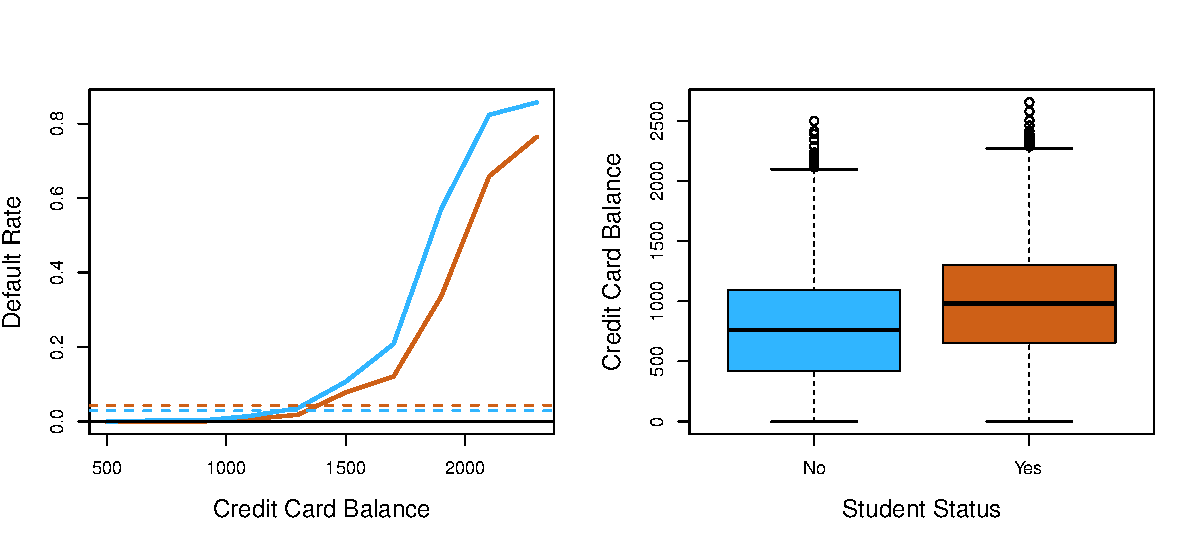
\includegraphics[scale=0.5]{figures/student}

This illustrates the dangers associated  with performing  regressions involving
only a single predictor  when other predictors may also be relevant.  As in
the linear regression setting, the results obtained using one predictor may be
quite different from those obtained using  multiple predictors, especially when there is correlation among the predictors.
}

\frame
{\frametitle{References}
\begin{itemize}
\item James G., Witten D., Hastie T., Tibshirani R. (2013), \textit{An introduction to Statistical Learning}$^*$, Springer.
\item Wei Y. (2016) Visualization Notes,  Plymouth University.
\item GGplot2 Cheat Sheet, \url{https://www.rstudio.com/wp-content/uploads/2015/03/ggplot2-cheatsheet.pdf}
\end{itemize}

\vspace{1cm}

$^*$ {\tiny Some of the figures in this presentation are taken from``An Introduction to Statistical Learning, with applications in R"  (Springer, 2013) with permission from the authors: G. James, D. Witten,  T. Hastie and R. Tibshirani.}
}

%\section{Project List}
%\frame{
%\frametitle{Statistics Project List}
%
%\begin{enumerate}
%  \item Diabetes
%  \item Airfoil Self-Noise Prediction
%  \item Concrete Compressive Strength
%  \item Energy Efficiency
%\end{enumerate}
%}

\frame{

\frametitle{Progress Checklist}

\begin{itemize}
  \item Start now!
  \item Study your project
  \item Read relevant chapters in the recommended books
  \item Using R, produce graphs and apply statistical learning methods to your project
  \item Understand the underlying methods
  \item Be able to interpret your results
  \item Write up your presentation slides...practice your presentation... and finally write up your scientific report
\end{itemize}
}



\endgroup
%----------------------------------------------------------------------------------------
\end{document} 